\begin{question}
\noindent Shape $S$ is drawn on the grid below.

\begin{center}
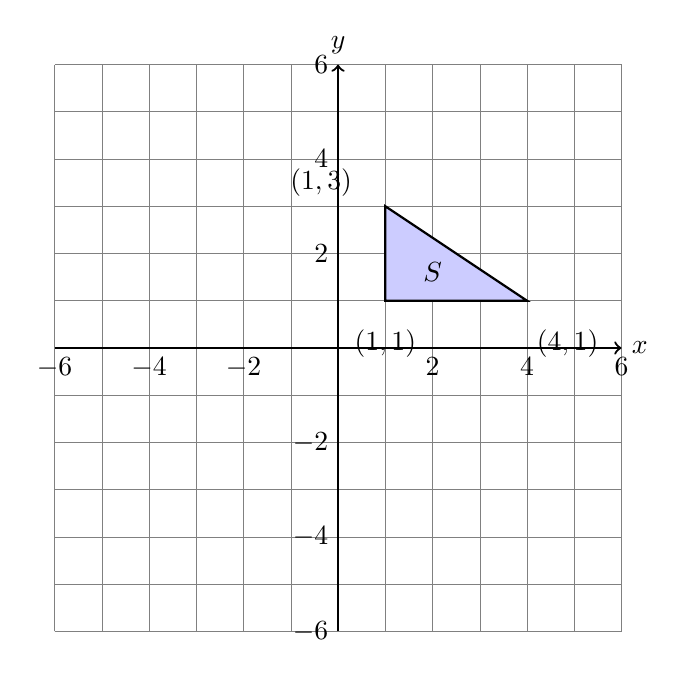
\begin{tikzpicture}[scale=0.6]
    % Grid
    \draw[step=1cm,gray,very thin] (-6,-6) grid (6,6);
    % Axes
    \draw[thick,->] (-6,0) -- (6,0) node[right] {$x$};
    \draw[thick,->] (0,-6) -- (0,6) node[above] {$y$};

    % Axis number labels
    \foreach \x in {-6,-4,-2,2,4,6}
        \node[below] at (\x,0) {$\x$};
    \foreach \y in {-6,-4,-2,2,4,6}
        \node[left] at (0,\y) {$\y$};

    % Shape S: right-angled triangle with vertices (1,1), (4,1), (1,3)
    \draw[thick, fill=blue!20] (1,1) -- (4,1) -- (1,3) -- cycle;
    \node at (1,0.6) [below] {$(1,1)$};
    \node at (4,0.6) [below right] {$(4,1)$};
    \node at (0.5,3) [above left] {$(1,3)$};
    \node at (2,1.6) {$S$};
\end{tikzpicture}
\end{center}

\noindent Rotate shape $S$ by $90^\circ$ clockwise about the origin $O$.

\noindent Draw and label the image $S'$ on a copy of the grid, and state the coordinates of the vertices of $S'$.

\vspace{4cm}

\begin{flushright}
\answerplain{2}
\end{flushright}
\end{question}
